\section{Theorie}
\label{sec:Theorie}

% In knapper Form sind die physikalischen Grundlagen des Versuches, des Messverfahrens, sowie sämtliche für die Auswertung erforderlichen Gleichungen darzustellen. (Keine Herleitung)

% (eventuell die Aufgaben)

% Der Versuchsaufbau: Beschreibung des Versuchs und der Funktionsweise (mit Skizze/Bild/Foto)

Wenn eine Masse $m$ bewegt werden soll, muss zunächst die Trägheit dieser Masse überwunden werden. Das Trägheitsmoment $I$ ist dabei äquivalent bei einer Drehbewegung, eine Trägheit, die überwunden werden muss, bevor ein Körper rotieren kann. Dabei ist das Trägheitsmoment einer Punktmasse

\begin{equation}
    I = m \cdot r^2.
    \label{eq:trägheit1}
\end{equation}

Dabei ist $m$ die Masse der Punktmasse und $r$ der senkrechte Abstand zur Rotationsachse. Weiterhin können die Trägheitsmomente von verschiedenen Masseelementen zu 

\begin{equation}
    I = \sum _i m_i \cdot r_i^2
    \label{eq:trägheit1}
\end{equation}

addiert werden. Äquivalent dazu kann das Trägheitsmoment infinitismaler Massen über 

\begin{equation}
    I = \int r^2 \dif{m}
    \label{eq:trägheit2}
\end{equation}

bestimmt werden. Bei bekannter Dichte $\rho$ und dem Volumen $V$ kann \autoref{eq:trägheit2} und über den Zusammenhang

\begin{equation}
    m = \rho \cdot V,
    \label{eq:dichte}
\end{equation}

in die Form 

\begin{equation}
    I = \int r^2 \cdot \rho \dif{V}
    \label{eq:trägheit2}
\end{equation}

gebracht werden. So ist das Trägheitsmoment eines Zylinders durch \autoref{fig:zylinder} gegeben.

\begin{figure}
    \centering
    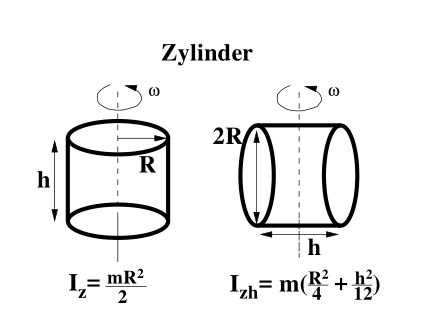
\includegraphics[width=\textwidth/2]{images/zylinder.png}
    \caption{Trägheitsmoment eines Zylinders um zwei seiner Hauptachsen \cite{V101}}
    \label{fig:zylinder}
\end{figure}

Ein Körper hat immer einen Schwerpunkt $m_\text{S}$, durch den drei Schwerpunktsachsen gelegt werden können. 
Sind die Trägheitsmomente dieser Achsen bekannt, können die Trägheitsmomente aller zu ihnen parallelen Achsen durch den Satz von Steiner bestimmt werden. 
Dafür müssen die Masse $m$ des Körpers, der senkrechte Abstand $r$ der beiden Achsen und der Schwerpunktsträgheitsmoment $I_\text{S}$ bekannt sein. Es ergibt sich der Zusammenhang 

\begin{equation}
    I = I_\text{S} + m \cdot r^2.
    \label{eq:steiner}
\end{equation}

Wird ein drehbarer Körper mit einer Kraft $F$ im Abstand $r$ von der Drehachse ausgelenkt, wirkt auf ihn ein Drehmoment

\begin{equation}
    M = F \times r.
    \label{eq:drehmoment}
\end{equation}

Sollte das System schwingungsfähig sein, und wird um den Winkel $\varphi$ ausgelenkt, wirkt das rücktreibende Drehmoment, hier durch eine Feder, der Drehung entgegen. Die daraus resultierende harmonische Schwingung mit der Periodendauer $T$ ist dann

\begin{equation}
    T = 2\pi \cdot \sqrt{\frac{I}{D}}.
    \label{eq:schwingung}
\end{equation}

Das Trägheitsmoment $I$ setzt sich aus der Trägheit des rotierenden Objektes $I$ und der Eigenträgheit der Drillachse $I_\text{D}$ zusammen. $D$ wird als Winkelrichtgröße bezeichnet und ist als 

\begin{equation}
    D = \frac{M}{\varphi} = \frac{F \cdot r}{\varphi}
    \label{eq:winkelrichtgröße}
\end{equation}

definiert. 